\chapter{Technical Background}

This chapter will cover the following preliminary topics: cryptographic primitives, isogenies and their relevant properties, supersingular isogeny Diffie-Hellman (SIDH), the Fiat-Shamir construction for digital signatures (and its quantum-safe adaptation), the current landscape of isogeny-based signature schemes, and finally select C implementations of the isogeny-based protocols with which we are concerned.

In the first section of this chapter we will take some time to introduce a few ideas from modern cryptography. We will cover key exchange, identification schemes, and signature schemes - all at as high of an abstraction level as possible. Readers familiar with these topics can skip this section without harm. 

Our discussion of isogenies will begin with some basic coverage of the underlying algebra. We will provide the material necessary for the remaining sections as we build up in the level of abstraction; working our way through groups, finite fields, elliptic curves, and finally isogenies and their properties.

Once we have presented the necessary algebra, we will illustrate the specifics of the supersingular isogeny Diffie-Hellman key-exchange protocol. We will spend most of this time dedicated to a modular deconstruction of the protocol, looking at the high-level procedures and algorithms which will be necessary for understanding in detail the signature protocol to come. This subsection will end with a briefing and analysis of the closely related zero-knowledge proof of identity (ZKPoI) protocol proposed in the original De Feo et al. paper \cite{djp}, as it is the foundation for the isogeny-based signature scheme presented by Yoo et al \cite{yoo}.

In section 2.3 we will discuss the Fiat-Shamir transformation \cite{sigs}; a technique which, given a secure interactive identification scheme, creates a secure digital signature scheme. We will also look at the quantum-secure adaptation published by Unruh \cite{unruh}, as applying a non-quantum-resistant transform to a quantum-resistant primitive would be rather frivolous.

Section 2.4 will be dedicated to covering current isogeny-based signature schemes - the topic about which this dissertation is mainly concerned. We will discuss the signature scheme of Yoo et al., which is a near direct application of Unruh's work to the SIDH zero-knowledge proof of identity.

Finally, the last section of this chapter will introduce the SIDH C library released by Microsoft Research, on top of which the core contributions of this thesis are implemented. We will also look at the implementation of the to-be-discussed signature scheme, which is a proof-of-concept built on top of the Microsoft API.\\


\section{Cryptographic Primitives}
\label{sec:crypto}

Cryptographic primitives can be thought of as the basic building blocks of cryptographically secure applications and protocols. The idea of which being that if individual primitives are provably (or believeably) secure, we can be more confident in the security of the application as a whole.\footnote{This is not to say that software which implements provably secure primitives is guaranteed to be secure. In security, it should be expected that the weakest link in the system is the first to be exploited, and these weak links often lie in careless implementation details.}

To quickly recap some basic information security, there are serveral different security properties a cryptographic primitive may aim to offer:
\begin{itemize}
\item \emph{Confidentiality}:
The notion that the information in question is kept private from unauthorized individuals.
\item \emph{Integrity}:
The notion that the information in question has not been altered by unauthorized individuals.
\item \emph{Availability}:
The notion that the information in question is available to authorized individuals when requested.
\item \emph{Authenticity}:
The notion that the source of the information in question is verified.
\item \emph{Non-repudiation}:
The notion that the source of the information in question \textbf{cannot} deny having originally provided the information.
\end{itemize}

The security of a particular cryptographic primitive is measured by two components. The first, referred to often as a ``security guarantee", measures what conditions constitute a successful attack on the primitive. The second, known as the ``threat model", makes assumptions about the computational powers that the adversary holds. The best practice in forming security proofs is to aim for security with respect to the most easily broken security guarantee and the most challenging possible threat model. The combination of a security guarantee and threat model is known as a \emph{security goal}.

Each of the primitives to come are designed to offer some security to the communication between a given pair of entities. We will refer to these entities as Alice and Bob. The schemes we are concerned with in this dissertation are strictly \emph{public key} (also known as \emph{asymmetric key}) schemes. In public key primitives, each user possesses a \emph{public} key (visible to every user in the network) as well as a \emph{private} key, which only they have access to. 

The first class of primitives we will discuss, \emph{key exchange} protocols, provide a means by which Alice and Bob can come to the agreement of some secret value. The goal of a key exchange protocol is for Alice and Bob, communicating over some open, insecure channel, to reach mutual agreement of the secret value while also ensuring the \emph{confidentiality} of that value. The secret value is referred to as a \emph{secret} or \emph{shared} key and is intended for use in other cryptographic primitives. 

Identification schemes are a class of primitives that aim to ensure \emph{authenticity} of a given entity. If Alice is communicating with Bob and she wants to verify that Bob is who he claims to be, the two can utilize a secure identification scheme. After identification protocols we will look at signature schemes, which are somewhat of an extension of the former. Signature schemes aim to provide \emph{authenticity} on every message sent from Bob to Alice, as well as \emph{non-repudiability} and \emph{integrity} of those messages.\\

\noindent
\emph{Random Oracle Model}. Before continuing with our discussion of primitives, it is worth covering briefly a framework in cryptography known as the random oracle model. A ``random oracle" is a theoretical black box which, for every unique input, responds with a truly random output. That is, if a query is made to a random oracle $h$ with input $x$ (written $h(x)$) multiple times, $h$ with respond with the same (random) output every time.

For certain constructions to be proven secure, it is sometimes necessary or helpful to assume the existence of random oracles. While this assumption may seem greviously optimistic, \emph{hash functions} are a widely diployed family of functions which are believed to approach the nature of random oracles to some degree. Much of the security of modern cryptography depends on the security of such hash functions.

\subsection{Key Exchange}

A key exchange protocol, which we will denote as $\Pi_{kex}$, can be represented in some contexts by a pair of polynomial time algorithms \textbf{KeyGen} and \textbf{SecAgr}: $\Pi_{kex} = (\textbf{KeyGen},\textbf{SecAgr})$. Alice and Bob will each run both of these procedures. The first they will run on the same input, $1^\lambda$, a bit string of $\lambda$ 1's. The second, short for ``secret agreement'', they will run on both their outputs of \textbf{KeyGen} and their peers.\\

Execution of $\Pi_{kex}$ between Alice and Bob involves the following:
\begin{enumerate}[label=(\roman*)]
\item Alice and Bob run $\textbf{KeyGen}(1^\lambda)$: A probabilistic algorithm with input $1^\lambda$ and output $(sk,pk)$. Typically $pk$ is the image of $f(sk)$, where $f$ is some \emph{one-way} function. We will denote the outputs of \textbf{KeyGen} for Alice and Bob as $(sk_{\text{Alice}},pk_{\text{Alice}})$ and $(sk_{\text{Bob}},pk_{\text{Bob}})$ respectively.
\item Alice and Bob exchange (over an insecure channel) their public keys $pk_{\text{Alice}}$ and $pk_{\text{Bob}}$.
\item Alice runs $\textbf{SecAgr}(sk_{\text{Alice}}, pk_{\text{Bob}})$: A deterministic algorithm with input $sk_{\text{Alice}}$ and $pk_{\text{Bob}}$ and output $k_{\text{Alice}} \in \{0,1\}^\lambda$. Bob runs $\textbf{SecAgr}(sk_{\text{Bob}}, pk_{\text{Alice}})$ to obtain $k_{\text{Bob}} \in \{0,1\}^\lambda$.
\end{enumerate}

\begin{figure}[!ht]
\begin{center}
\begin{tikzpicture}
  % Public parameter:
  \node[draw=none,fill=none,align=center] (public) at (0,1) {Public parameter:\\$g, p$};
  
  % Alice
  \node[draw] (Alice) at (-2,0) {Alice}; 
  \draw[thick] (Alice) -- ++(0, -4);
    
  % Calculations of Alice
  \node[draw=none,fill=none,anchor=east] (asecret) at ($(Alice) + (0,-1)$) {$a \in_{R} \{2,\dots,p-2\}$};
  \node[draw=none,fill=none,anchor=east] (Apublic) at ($(Alice) + (0,-2)$) {$A = g^{a} \bmod{p}$};
  \node[draw=none,fill=none,anchor=east] (akey) at ($(Alice) + (0,-4)$) {$k = (B)^{a} = g^{ba}$};
    
  % Bob
  \node[draw] (Bob) at (2,0) {Bob}; 
  \draw[thick] (Bob) -- ++(0, -4);
   
  % Calculations of Bob
  \node[draw=none,fill=none,anchor=west] (bsecret) at ($(Bob) + (0,-1)$) {$b \in_{R} \{2,\dots,p-2\}$};
  \node[draw=none,fill=none,anchor=west] (Bpublic) at ($(Bob) + (0,-2)$) {$B = g^{b} \bmod{p}$};
  \node[draw=none,fill=none,anchor=west] (bkey) at ($(Bob) + (0,-4)$) {$k = (A)^{b} = g^{ab}$};
   
  % Messages
  \draw[->,thick] ($(Alice)+(0,-2)$) -- ($(Bob)+(0,-2.5)$) node [pos=0.5,above,font=\footnotesize] {A};
  \draw[->,thick] ($(Bob)+(0,-3)$) -- ($(Alice)+(0,-3.5)$) node [pos=0.5,above,font=\footnotesize] {B};
    
\end{tikzpicture}
\end{center}
\caption{Alice and Bob's execution of Diffie-Hellman key exchange.}
\label{fig:diffiehellman}
\end{figure}

\noindent
$\Pi_{kex}$ is said to uphold \emph{correctness} if $k_{Alice} = k_{Bob}$ for all honestly derived keypairs $(sk_{\text{Alice}},pk_{\text{Alice}})$ and $(sk_{\text{Bob}},pk_{\text{Bob}})$. Because we deal only with correct $\Pi_{kex}$, we refer to the output of $\Pi_{kex}$ as simply $k$. 

Figure \ref{fig:diffiehellman} illustrates an execution of the Diffie-Hellman key exchange protocol which relies on the difficulty of the \emph{discrete logarithm} problem for its one-way function $f$.\\

The security goal typical of a key exchange protocol is that an adversary with access to the session transcript (threat) cannot discern the resulting shared secret key from a randomly generated value (security guarantee).

\subsection{Interactive Identification Schemes}

Imagine Alice wishes to confirm the identity of Bob. The motivation for interactive identification schemes is to provide Bob with some mechanism for proving to Alice (or any other party) that he has knowledge of some secret which \textbf{only} Bob could possess. The goal, of course, being to accomplish this without openly revealing the secret, so that it can continue to be used as an identifier for Bob. 

An identification scheme (or otherwise ``proof of identity" protocol) $\Pi_{id}$ is composed of by the tuple of polynomial-time algorithms (\textbf{KeyGen}, \textbf{Commit}, \textbf{Prove}, \textbf{Verify}) and some set $\omega$. $\Pi_{id}$ is an interactive protocol requiring two parties. The \emph{prover} (Bob, for example) executes \textbf{KeyGen}, \textbf{Commit}, and \textbf{Prove}. The \emph{verifier} (Alice, in our example) executes \textbf{Verify} following Bob's actions. 

Execution of $\Pi_{id}$ between Alice and Bob proceeds as follows:
\begin{enumerate}[label=(\roman*)]
\item Bob runs \textbf{KeyGen($1^\lambda)$}: A probabilistic algorithm with input $1^\lambda$ and outputs Bob's keypair $(sk,pk)$. Bob sends his public key $pk$ to Alice.
\item Bob runs \textbf{Commit()}: a probabilistic algorithm with output $com$. $com$ is referred to as a ``commitment". Bob sends $com$ to Alice.
\item Alice sends a randomly generated ``challenge" value $ch \in \omega$. Alice sends $ch$ to Bob. 
\item Bob runs \textbf{Prove($sk$, $com$, $ch$)}: A deterministic algorithm with input $sk$ and $ch$, and output $resp$. $resp$ is the ``response" to Alice's challenge.
\item Alice runs \textbf{Verify($pk$, $com$, $ch$, $resp$)}: A deterministic algorithm with input $pk$, $com$, $ch$, and $resp$, and output $b \in {0,1}$. Bob has successfully proven his identity to Alice if $b = 1$.
\end{enumerate}

\begin{figure}[!h]
\begin{center}
\begin{tikzpicture}
  % prover
  \node[draw] (prover) at (-2,0) {$\mathcal{P}$}; 
  \draw[thick] (prover) -- ++(0, -5);
    
  % Calculations for the prover
  \node[draw=none,fill=none,anchor=east] (asecret) at ($(prover) + (0,-1)$) {$(sk, pk) =$ \textbf{KeyGen($1^\lambda)$}};
  \node[draw=none,fill=none,anchor=east] (Apublic) at ($(prover) + (0,-2)$) {$com =$ \textbf{Commit()}};
  \node[draw=none,fill=none,anchor=east] (akey) at ($(prover) + (0,-4)$) {$resp =$ \textbf{Prove($sk$, $com$, $ch$)}};
    
  % verifier
  \node[draw] (verifier) at (2,0) {$\mathcal{V}$}; 
  \draw[thick] (verifier) -- ++(0, -5);
   
  % Calculations for the verifier
  \node[draw=none,fill=none,anchor=west] (Bpublic) at ($(verifier) + (0,-2.5)$) {$ch \gets_{R} \omega$};
  \node[draw=none,fill=none,anchor=west] (bkey) at ($(verifier) + (0,-4.5)$) {$b =$ \textbf{Verify($pk$, $com$, $ch$, $resp$)}};
   
  % Messages
  \draw[->,thick] ($(prover)+(0,-2)$) -- ($(verifier)+(0,-2.5)$) node [pos=0.5,above,font=\footnotesize] {$pk, com$};
  \draw[->,thick] ($(verifier)+(0,-3)$) -- ($(prover)+(0,-3.5)$) node [pos=0.5,above,font=\footnotesize] {$ch$};
  \draw[->,thick] ($(prover)+(0,-4)$) -- ($(verifier)+(0,-4.5)$) node [pos=0.5,above,font=\footnotesize] {$resp$};
    
\end{tikzpicture}
\end{center}
\caption{A general interactive identification scheme with prover $\mathcal{P}$ and verifier $\mathcal{V}$.}
\label{fig:piid}
\end{figure}

If Alice accepts Bob's response, and $b = 1$, then we refer to the tuple $(com,ch,resp)$ as an \emph{accepting transcript}. This general construction for identification protocols is illustrated in Figure \ref{fig:piid}, where the prover is referred to as $\mathcal{P}$ and $\mathcal{V}$ denotes the verifier.

In terms of security, it is common to show that an identification scheme is secure against \emph{impersonation} under a \emph{passive attack}. Proving such security implies that an adversary who eavesdrops on arbitrarily many executions of $\Pi_{id}$ between a verifier $\mathcal{V}$ and a prover $\mathcal{P}$ cannot successfully impersonate $\mathcal{V}$.\\

\noindent
We may at times speak of \emph{canonical} identification schemes. An identification scheme $\Pi$ occuring between a prover $\mathcal{P}$ and a verifier $\mathcal{V}$ is labelled canonical if it satisfies all of the following constraints:
\begin{itemize}
\item $\Pi$ consists of an initial message (or ``commitment") $com$ sent by $\mathcal{P}$, a challenge $ch$ sent by $\mathcal{V}$, and a final response $resp$ sent by $\mathcal{P}$.
\item $ch$ is chosen uniformly at random from some set $\omega$.
\item $com$ is generated by some probabilistic function \textbf{R} taking $\mathcal{P}$'s secret key as input. For any secret key $sk$ and fixed string $\bar{com}$, the probability that \textbf{R($sk$)} $= \bar{com}$ is negligible. 
\end{itemize}

These constraints gurantee that $\Pi$ will have two important features. First, that any third party given the transcript and prover's public key can efficiently determine whether the verifier will accept. Second, that the probability that $comm$ repeats in polynomially many executions of $\Pi$ is negligible.  

Lastly, it should be mentioned that there exist variations upon this type of primitive wherein Alice is not required to send Bob a specific challenge value. These are known as \emph{non-interactive} identification schemes, or non-interactive proofs of identity (NIPoI). These non-interactive approaches to solving the problem of identity and \emph{authentication} further bridge the gap between identification protocols and signature schemes. 

\subsection{Signature Schemes}

We define a signature scheme as the tuple of algorithms $\Pi_{sig}$ = (\textbf{KeyGen}, \textbf{Sign}, \textbf{Verify}). Some execution of $\Pi_{sig}$ between Alice and Bob for a particular message $m$ sent from Bob to Alice involves the following...
\noindent
First, before any message is to be signed, the Bob must run the following:
\begin{itemize}
\item Bob runs $\textbf{KeyGen}(1^\lambda)$: A probabilistic algorithm with input $1^\lambda$ and output $(sk,pk)$.
\end{itemize}
Then, for every message $m$ Bob wishes to authenticate and send to Alice: 
\begin{enumerate}[label=(\roman*)]
\item Bob sends his public key $pk$ to Alice over an authenticated channel if he has not yet done so.
\item Bob runs $\textbf{Sign}(sk, m)$: A probabilistic algorithm with input $sk$ (Bob's secret key) and $m$ (the message Bob wishes to authorize) and output $\sigma$, known as a \emph{signature}.
\item Bob sends $m$ and $\sigma$ to Alice.
\item Alice runs $\textbf{Verify}(pk, m, \sigma)$: A deterministic algorithm with input $pk$ (Bob's public key), $m$, and $\sigma$ and output $b \in \{0,1\}$. Alice has confidence in the \emph{integrity} and origin \emph{authenticity} of $m$ if $b = 1$.
\end{enumerate}

As previously alluded to, it is worth noting that signature protocols and identification schemes are closely related. In essence, they are rather similar; but with two main differences. The first is rather comparable to the aforementioned difference between interactive identification schemes and non-interactive identification schemes. The second arises as a result of aiming to authenticate Bob on any particular message $m$. To achieve this, the signature scheme needs to be run every time Bob wishes to send a message to Alice. The details of this comparison are intentionally left vague, as it will from a topic of close inspection in section 2.4.

The strongest security goal for a signature scheme $\Pi_{sig}$ is expressed as \emph{existential unforgeability} under an \emph{adaptive chosen-message attack}. If this goal is provably satisfied, an adversary with the ability to sign arbitrary messages will not be able to forge any conceivable and valid signature.

\section{Algebraic Geometry \& Isogenies}
\emph{Groups \& Varieties}. A \textbf{group} is a 2-tuple composed of a set of elements and a corresponding group operation (also referred to as the group \emph{law}). Given some group defined by the set $G$ and the operation $\cdot$ (written as $(G,\cdot)$) it is typical to refer to the group simply as $G$. If $\cdot$ is equivalent to some rational mapping\footnote{A rational map is a mapping between two groups which is defined by a polynomial function with rational coefficients.} $f_G: G \rightarrow G$, then the group $(G,\cdot)$ is said to form an \textbf{algebraic variety}. A group which is also an algebraic variety is referred to as an \textbf{algebraic group}.

$G$ is said to be an \emph{abelian} group if, in addition to the four traditional group axioms (closure, associativity, existence of an identity, existence of an inverse), $G$ satisfies the condition of commutitiviy. More formally, for some group $G$ with group operation $\cdot$, we say $G$ is an abelian group iff $x \cdot y = y \cdot x$ $\forall x, y \in G$. An algebraic group which is also abelian is referred to as an \textbf{abelian variety}.

\begin{tcolorbox}
\begin{definition}[Abelian Variety]
\label{defn:abelianvariety}
for some algebraic group $G$ with operation $\cdot$, we say $G$ is an \underline{abelian variety} iff $x \cdot y = y \cdot x$ $\forall x, y \in G$. 
\end{definition}
\end{tcolorbox}

For some group $(G,\cdot)$, some $x,y \in G$, and some rational mapping $f_G: G \rightarrow G$, let the following sequence of implications denote the classification of $(G,\cdot)$:

$$
\text{group } \xRightarrow[]{x\cdot y = f_G(x,y)} \text{algebraic group } \xRightarrow[]{x\cdot y = y\cdot x} \text{abelian variety }
$$

\noindent
\emph{Morphisms}. Let us again take for example some group $(G,\cdot)$. Let's also define some set $S_{(G,\cdot)}$ which contains every tuple $(x,y,z)$ for group elements $x,y,z$ which satisfy $x\cdot y = z$.
$$
S_{(G,\cdot)} = \{x,y,z \in G | x\cdot y = z\}
$$
Take also for example a second group $(H,*)$ and some map $\phi: G \rightarrow H$. $\phi$ is said to be \emph{structure preserving} if the following implication holds:
$$
(x,y,z) \in S_{(G,\cdot)} \Rightarrow (\phi(x),\phi(y),\phi(z)) \in S_{(H,*)}
$$

A \textbf{morphism} is simply the most general notion of a structure preserving map. More specifically, in the domain of algebraic geometry, we will be dealing with the notion of a \textbf{group homomorphism}, defined as follows:
\begin{tcolorbox}
\begin{definition}[Group Homomorphism]
\label{defn:homomorphism}
For two groups $G$ and $H$ with respective group operations $\cdot$ and $*$, a \underline{group homomorphism} is a structure preserving map $h: G \rightarrow H$ such that $\forall u, v \in G$ the following holds:
$$h(u \cdot v) = h(u) * h(v)$$
\end{definition}
\end{tcolorbox}

From this simple definition, two more properties of homomorphisms are easily deducible. Namely, for some homomorphism $h: G \rightarrow H$, the following properties hold:
\begin{itemize}
\item $h$ maps the identity element of $G$ onto the identity element of $H$, and
\item $h(u^{-1}) = h(u)^{-1}, \forall u \in G$
\end{itemize}
Recall that for some morphism (or function) $h: G \rightarrow H$, we refer to $G$ as the domain and $H$ as the codomain.

Furthermore, an \emph{endomorphism} is a special type of morphism in which the domain and the codomain are the same groups. We denote the set of enomorphisms defineable over some group $G$ as $\text{End}(G)$.
The \emph{kernel} of a particular homomorphism $h: G \rightarrow H$  is the set of elements in $G$ that, when applied to $h$, map to the identity element of $H$. We write this set as $ker(h)$, and it is much analogous to the familiar concept from linear algebra, wherein the kernel denotes the set of elements mapped to the zero vector by some linear map.
\vspace{10mm}

\subsection{Fields \& Field Extensions}
\label{subsec:fields}

A \textbf{field} is a mathematical structure which, while being similar to a group, demands additional properties. Fields are defined by some set $F$ and two operations: \emph{addition} and \emph{multiplication}. In order for some tuple $(F,+,\cdot)$ to constitute a field, it must satisfy an assortment of axioms:\\

\emph{Addition axioms}:
\begin{itemize}
\item (closure) If $x \in F$ and $y \in F$, then $x + y \in F$.
\item $+$ is commutative.
\item $+$ is associative.
\item $F$ contains an element 0 such that $\forall x \in F$ we have $0 + x = x$.
\item $\forall x \in F$ there is a corresponding element $-x \in F$ such that $x + (-x) = 0$.
\end{itemize}

\emph{Multiplication axioms}:
\begin{itemize}
\item (closure) If $x \in F$ and $y \in F$, then $x \cdot y \in F$.
\item $\cdot$ is commutative.
\item $\cdot$ is associative.
\item $F$ contains an element $1 \neq 0$ such that $\forall x \in F$ we have $x \cdot 1 = x$.
\item $\forall x \neq 0 \in F$ there is a corresponding element $x^{-1} \in F$ such that $x \cdot (x^{-1}) = 1$.
\end{itemize}

Additionally, a field $(F,+,\cdot)$ must uphold the \emph{distributive law}, namely:
$$
 x \cdot (y + z) = x \cdot y + x \cdot y \text{ holds } \forall x,y,z \in F
$$

While these axioms are known to be satisfied by the sets $\mathbb{Q}$, $\mathbb{R}$, and $\mathbb{C}$ with typically defined $+$ and $\cdot$, our focus will be on a particular class of field known as a \emph{finite field}. Finite fields, as the name suggests, are fields in which the set $F$ contains finitely many elements - we refer to the number of elements in $F$ as the \emph{order} of the field.

Let us take some prime number $p$. We can construct a finite field by taking $F$ as the set of numbers $\{0, 1, ... p-1\}$ and defining $+$ and $\cdot$ as addition and multiplication \emph{modulo p}. Finite fields defined in this fashion are denoted as $\mathbb{F}_p$, and have order $p$.
\begin{center}
$\forall x,y \in \mathbb{F}_p$, $x + y = (x + b) \mod{p}$, and\\
$\forall x,y \in \mathbb{F}_p$, $x \cdot y = (x \cdot b) \mod{p}$\\
\end{center}

For any given field $K$ there exists a number $q$ such that, for every $x \in K$, adding $x$ to itself $q$ times results in the additive identity 0. This number is referred to as the \emph{characteristic} of $K$, for which we write char($K$). Finite fields are the only type of field for which $\text{char}(K) > 0$. Furthermore, if the field in question is finite and has prime order, then the order and the characteristic are equivalent.

A particular field $K'$ is called an \emph{extension field} of some other field $K$ if $K \subseteq K'$. The complex numbers $\mathbb{C}$, for example, are an extension field of $\mathbb{R}$. A given field $K$ is \emph{algebraically closed} if there exists a root for every non-constant polynomial defined over $K$. If $K$ itself is not algebraically closed, we denote the extension of $K$ that is by $\overline{K}$. 

An algebraic group $G_a$ is defined over a field $K$ if each element $e \in G_a$ is also an element of the field $K$, and the corresponding $f_{G_a}$ is defined over $K$. To show that a particular algebraic group $G_a$ is defined over some field $K$ we will henceforth denote the group/field pairing as $G_a(K)$. Naturally, in the case where our field is a finite field of order $p$, we write $G_a(\mathbb{F}_p)$.

These algebraic structures are all important for building up to the concept of an \emph{isogeny}. The lowest-level object we will be concerned with when discussing the forthcoming isogeny-based protocols will typically be elements of abelian varieties. The lowest-level structure in the SIDH C codebase is a finite field element.\\

\noindent
\emph{Montgomery Arithmetic}\label{snip:montgomery}. We will now briefly discuss a technique for efficiently performing modular arithmetic. This method is widely deployed in cryptosystems centered around finite fields, and is abundantly used in the \sidh library that we will shortly be examining.

In 1985, Peter Montgomery introduced a method for efficiently computing the modular multiplication of two elements $a$ and $b$. The technique begins with the construction of some constant $R$, whose value depends solely on the modulus $N$ and the underlying computer architecture.\footnote{The specifics of how $R$ is constructed are beyond the scope of this dissertation; if they feel so inclined, the reader should refer to \cite{mont}.}

With the retrieval of $R$, $aR \mod{N}$ and $bR \mod{N}$ are constructed and referred to as the Montgomery \emph{representation} of $a$ and $b$ respectively. Montgomery multiplication outlines an algorithm for computing $abR \mod{N}$ (the Montgomery product of $a$ and $b$), from which $ab \mod{N}$ can be recovered through conversion back to standard representation. Once in Montgomery representation, other arithmetic can be performed (including field element inversions) in order to leverage the performance improvement offered by Montgomery modular multiplication -- converting back to regular representation when necessary.

Applying Montgomery multiplication has the added benefit of decreasing the amount of field element inversions that need to be computed. Because of this, the technique is particularly relevant to this dissertation. We continue this discussion in section \ref{sec:pbinvimplementation}.

\subsection{Elliptic Curves}

An elliptic curve is an algebraic curve defined over some field $K$, the most general representation of which is given by
$$
y^2 + a_{1}xy + a_{3}y = x^3 + a_{2}x^2 + a_{4}x + a_6.
$$
This representation encapsulates elliptic curves defined over any field. If, however, we are dicussing curves defined specifically over a field $K$ such that $\text{char}(K) > 3$\footnote{See \cite{silverman}.}, then the more compact form $y^2 = x^3 + ax + b$ can be applied (see Figure \ref{fig:groupop} for a geometric visualization). In this dissertation we will default to this second representation, as the schemes with which we are concerned will always be defined over $\mathbb{F}_p$ for some large prime $p$.

We can define a group structure over the points of a given elliptic curve (or any other smooth cubic curve). If we wish to define a group in accordance to a particular curve, we do so with the following notation:
$$
E: y^2 = x^3 + ax + b
$$
Wherein $E$ denotes the group in question, the elements of which are all the points (solutions) of the curve. Throughout much of this section, the words \emph{point} and \emph{element} can be used interchangeably.\\

\noindent
\emph{The Group Law}. The group operation we define for $E$, denoted $+$, is better understood geometrically than algebraically. Consider the following.

Given two elements $P$ and $Q$ of some arbitrary elliptic curve group $E$, we define $+$ geometrically as follows: drawing the line $L$ through points $P$ and $Q$, we follow $L$ to its third intersection on the curve (which is guaranteed to exist), which we will denote as $R = (x_R, y_R)$. We then set $P + Q = -R$, where $-R$ is the reflection of $R$ over the x-axis: $(x_R, -y_R)$. This descriptive definition of $+$ is suitable for all situations \emph{except} for when $L$ is tangent to $E$ or when $L$ is parallel to the y-axis. These cases will be covered in a short moment. See Figure \ref{fig:groupop} for an illustrated representation of this process.

\begin{figure}[!h]
\begin{tikzpicture}[scale=.75]
	\begin{scope}[xshift=5cm]
		%\draw[very thin,color=gray] (-3.9,-3.9) grid (3.9,3.9);  %background grid
		\draw[->] (-4.2,0) -- (4.2,0) node[right] {$x$};         %x-axis
		\draw[->] (0,-4.2) -- (0,4.2) node[above] {$y$};         %y-axis
		
		\plotcurve{-2}{2}
		
		\draw[fill] (-1.73,0.531) circle (0.1) node[right] {$P$};
		\draw[fill] (0.28,1.209) circle (0.1) node[right] {$Q$};
	\end{scope}
	
	\begin{scope}[xshift=17cm]
		%\draw[very thin,color=gray] (-3.9,-3.9) grid (3.9,3.9);  %background grid
		\draw[->] (-4.2,0) -- (4.2,0) node[right] {$x$};         %x-axis
		\draw[->] (0,-4.2) -- (0,4.2) node[above] {$y$};         %y-axis
		
		\plotcurve{-2}{2}
		
		\draw [] (-1.73,0.531) -- (1.564,1.642);
		\draw [dashed] (1.564,1.642) -- (1.564,-1.642);
		
		\draw[fill] (-1.73,0.531) circle (0.1) node[right] {$P$};
		\draw[fill] (0.28,1.209) circle (0.1) node[right] {$Q$};
		\draw[fill] (1.564,1.642) circle (0.1) node[right] {$R$};
		\draw[fill] (1.564,-1.642) circle (0.1) node[right] {$R' = P+Q$};
  \end{scope}
\end{tikzpicture}
\caption{$+$ acting over points $P$ and $Q$ of $y^2 = x^3 - 2x + 2$.}
\label{fig:groupop}
\end{figure}

The group operation $+$ is referred to as \emph{pointwise addition}. In order for $(E,+)$ to properly form a group under pointwise addition, it must satisfy the four group axioms:
\begin{itemize}
\item \emph{Closure}: Because elliptic curves are polynomials of degree of 3, we know any given line passing through two points $P$ and $Q$ of $E$ will pass through a third point $R$. The exceptions here are twofold. First, when $P = Q$ and thus our line is tangent to $E$, and second, when $Q = -P$ and our line is parallel with the y-axis. We resolve the first case nicely by defining $P + P$ by means of taking $L$ to be the line tangent to $E$ at point $P$. In the second case, $P + (-P)$, by group axiom, should yield the identity element of the group. We will define this element and resolve this issue below.  
\item \emph{Identity}: The identity element of elliptic curve groups, denoted as $\mathcal{O}$, is a specially defined point satisfying $P + \mathcal{O} = \mathcal{O} + P = P$, $\forall P \in E$. Because of the inclusion of this special element, we have that $\#(E(K))$ is equal to $1$ $+$ the number geometric points on $E$ defined over $K$. This of course is only a noteworthy claim when $K$ is a finite field (otherwise there are already infinitely many elements in $E$).
\item \emph{Associativity}: For all points $P$, $Q$, and $R$ in $E$, it must be the case ($(P + Q) + R = P + (Q + R)$) holds. It is rather easy to see visually why this is true for geometrically defined points in $E$ (see Figure \ref{fig:axioms}). Additionally, we can trivially show that this holds when any combination of $P$, $Q$, and $R$ are $\mathcal{O}$ by applying the axiom of the identity.
\item \emph{Inverse}: Due to the x-symmetry of elliptic curves, every point $P = (x_P, y_P)$ of $E$ has an associated point $-P = (x_P, -y_P)$. If we apply $+$ to $P$ and $-P$, $L$ assumes the line parrallel to the y-axis at $x = x_P$. As discussed above, in this case there is no third intersection of $L$ on $E$. In light of this, $\mathcal{O}$ can be thought of as a point residing infinitely far in both the positive and negative directions of the y-axis. $\mathcal{O}$ is equivalently referred to as the \emph{point at infinity} (see Figure \ref{fig:axioms}).\footnote{One might suspect that the inclusion of this (apparently) non-algebraic element $\mathcal{O}$ suggests that $+$ is not a rational-map. The operator $+$ \emph{can} be shown to be a rational-mapping if we define our elliptic curve groups in three-dimensional projective space.}
\end{itemize}

\begin{figure}[!h]
\begin{tikzpicture}[scale=.55]
	\begin{scope}[xshift=0cm]
		%\draw[very thin,color=gray] (-3.9,-3.9) grid (3.9,3.9);  %background grid
		\draw[->] (-4.2,0) -- (4.2,0) node[right] {$x$};         %x-axis
		\draw[->] (0,-4.2) -- (0,4.2) node[above] {$y$};         %y-axis
		
		\draw[] (-1.65,0.677) -- (2.00,1.414); 
		\draw[dashed] (-0.309,0.948) -- (-0.309,-0.948);
		\draw[] (-1.400,-1.207) -- (1.765,-0.454); 
		\draw[dashed] (1.765,-0.454) -- (1.765,0.454);
		
		\plotcurve{-3}{0}
		
		\draw[fill] (-1.65,0.677) circle (0.1) node[left] {$P$};
		\draw[fill] (2.00,1.414) circle (0.1) node[right] {$Q$};
		\draw[fill] (-0.309,0.948) circle (0.1) node[right] {};
		\draw[fill] (-0.309,-0.948) circle (0.1) node[right] {};
		\draw[fill] (-1.400,-1.207) circle (0.1) node[below] {$R$};
		\draw[fill] (1.765,-0.454) circle (0.1) node[right] {};
		\draw[fill] (1.765,0.454) circle (0.1) node[right] {$(P + Q) + R$};
	\end{scope}
	\begin{scope}[xshift=10cm]
		%\draw[very thin,color=gray] (-3.9,-3.9) grid (3.9,3.9);  %background grid
		\draw[->] (-4.2,0) -- (4.2,0) node[right] {$x$};         %x-axis
		\draw[->] (0,-4.2) -- (0,4.2) node[above] {$y$};         %y-axis
		
		\draw[] (2.00,1.414) -- (-1.400,-1.207);
		\draw[dashed] (-0.006,-0.132) -- (-0.006,0.132);
		\draw[] (-1.65,0.677) -- (1.765,-0.454);
		\draw[dashed] (1.765,-0.454) -- (1.765,0.454);
		
		\plotcurve{-3}{0}
		
		\draw[fill] (-1.65,0.677) circle (0.1) node[left] {$P$};
		\draw[fill] (2.00,1.414) circle (0.1) node[right] {$Q$};
		\draw[fill] (-1.400,-1.207) circle (0.1) node[below] {$R$};
		\draw[fill] (-0.006,-0.132) circle (0.1) node[right] {};
		\draw[fill] (-0.006,0.132) circle (0.1) node[right] {};
		\draw[fill] (1.765,-0.454) circle (0.1) node[right] {};
		\draw[fill] (1.765,0.454) circle (0.1) node[right] {$P + (Q + R)$};
	\end{scope}
	\begin{scope}[xshift=20cm]
		%\draw[very thin,color=gray] (-3.9,-3.9) grid (3.9,3.9);  %background grid
		\draw[->] (-4.2,0) -- (4.2,0) node[right] {$x$};         %x-axis
		\draw[->] (0,-4.2) -- (0,4.2) node[above] {$y$};         %y-axis
		
		\plotcurve{1}{1}
		
		\draw[dashed] (0.73,-4.492) -- (0.73,4.492);
		
		\draw[fill] (0.73,1.492) circle (0.1) node[right] {$P$};
		\draw[fill] (0.73,-1.492) circle (0.1) node[right] {$-P$};
  \end{scope}
\end{tikzpicture}
\caption{associativity illustrated on $y^2 = x^3 - 3x$ (left \& center) and $P + (-P) = \mathcal{O}$ illustrated for $y^2 = x^3 + x + 1$ (right).}
\label{fig:axioms}
\end{figure}

Of course, there are relatively simple formulas for algebraically defining point-wise addition and inverse computation. We have opted to describe these operations geometrically simply for ease of communication.

Additionally, we shorthand $\overbrace{P + P + ... + P}^{n}$ as $nP$, analogous to scalar multiplication.\\

Consequently, because groups defined over elliptic curves in this fashion are commutitive, they also constitute abelian varieties.

When referring to curves as abelian varieties defined over a field, we will write them as $E_{\alpha}(K)$, for some curve $E_{\alpha}$ and some field $K$. If we are only concerned with the geometric properties of the curve, or curves as distinct elements of some group structure, it will suffice to write $E_{\alpha}$. Moving forward from here, we will assume all general curves discussed are capable of definition over some finite field $\mathbb{F}_p$.\\

The $r$-\emph{torsion group} of $E$ is the set of all points $P \in E(\overline{\mathbb{F}}_q)$ such that $rP = \mathcal{O}$. We denote the $r$-torsion group of some curve as $E[r]$.\\

\noindent
\emph{Supersingular Curves}. An elliptic curve can be either \emph{ordinary} or \emph{supersingular}. There are several equivalent ways of defining supersingular curves (and thus the distinction between them and ordinary curves) in a general setting, but each of these goes well beyond our scope. In the context of curves defined over finite fiels, however, the following succinct definition holds:
\begin{tcolorbox}
\begin{definition}[Supersingular Curve]
\label{defn:supersingular}
Let $E$ be an elliptic curve defined over the finite field $\mathbb{F}_{p}$. $E$ is said to be \underline{supersingular} if $\#(E(\mathbb{F}_{p})) = p+1$.\footnote{Readers are welcomed to investigate \cite{pairings} for further details.}
\end{definition}
\end{tcolorbox}

For the remainder of this paper, unless otherwise noted, all elliptic curves in discussion will supersingular.\\ 

\noindent
\emph{Projective Space}\label{snip:projspace}. While elliptic curves are naturally defined in two-dimensional affine space, there are many benefits to expressing them through three-dimension projective coordinates. First and foremost, expressing curves in projective space allows us to reason geometrically about $\mathcal{O}$. This is done by defining a curve $E$ such that it resides in some two-dimension subspace of 3-space, the point $\mathcal{O}$ then resides at some point in 3-space outside of the residing plane of $E$. 

Representing a curve in 3-space requires some substitution of $x$ and $y$ coordinates, a typical forma for achieving this is the following:

$$
x = X/Z\quad
y = Y/Z\quad
Z = 1
$$

Such a representation of elliptic curve points offers more computationally efficient arithmetic over points. This is conceptually similar to the previously mentioned Montgomery arithmetic regarding finite field elements. Other substitutions offer different computational advantages, but the implementations we will discuss make use of this typical approach.

\subsection{Isogenies \& Their Properties}

\begin{tcolorbox}
\begin{definition}[Isogeny]
\label{defn:isogeny}
Let $G$ and $H$ be algebraic groups. An \underline{isogeny} is a morphism $h: G \rightarrow H$ possessing a finite kernel.
\end{definition}
\end{tcolorbox}

In the case of the above definition where $G$ and $H$ are abelian varieties (such as elliptic curves,) the isogeny $h$ is homomorphic between $G$ and $H$. Because of this, isogenies over elliptic curves (and other abelian varieties) inherit certain characteristics.\\
For an isogeny $h: E_{1} \rightarrow E_{2}$ defined over elliptic curves $E_1$ and $E_2$, the following holds:
\begin{itemize}
\item $h(\mathcal{O}) = \mathcal{O}$, and
\item $h(u^{-1}) = h(u)^{-1}, \forall u \in G$
\end{itemize}

If there exists some isogeny $\phi$ between curves $E_1$ and $E_2$ then $E_1$ and $E_2$ are said to be \emph{isogenous}. All supersingular curves are isogenous only to other supersingular curves. The equivalent statement holds for ordinary curves. With this in mind, we can concieve a sort of graph structure connecting all isogenous curves, these graphs pertaining to either the supersingular or ordinary variety of curves. 

We write $\text{End}(E)$ to denote the ring formed by all the isogenies acting over $E$ which are also endomorphisms. Note that $m$-repeated pointwise addition of a point with itself can equivalently be modelled by an endomorphism, we denote the application of such an endomorphism to a point $P$ as $[m]P$, such that $[m]: E \rightarrow E$ and $[m]P = mP$.

An important facet of isogenies is that they can be uniquely identified by their kernel. If $S$ is the group of points denoting the kernel of some isogeny $\phi$ with domain $E$, we write $\phi: E \rightarrow E/S$. Because the subgroup $S$ sufficiently identifies $\phi$, any given generator of $S$ equivalently identifies $\phi$. Therefore, if $R$ generates the subgroup $S$ we can write $\phi: E \rightarrow E/\langle R \rangle$. Moreover, we will have a specific interest in isogenies with kernels defined by some \emph{torsion subgroup}. 

\begin{tcolorbox}
\begin{lemma}[Uniquely identifying isogenies]
\label{lem:isogkern}
Let $E$ be an elliptic curve and let $\Phi$ be a finite subgroup of $E$. There are a unique elliptic curve $E'$ and a seperable isogeny $\phi: E \rightarrow E'$ satisfying $\text{ker}(\phi) = \Phi$.
\end{lemma}
\end{tcolorbox}

\section{Supersingular Isogeny Diffie-Hellman}
\label{sec:sidh}

This section will aim to accomplish two things. First, we will briefly explain the isogeny-level \& key-exchange-level procedures of the SIDH protocol. Second, we will illuminate how these procedures map onto Microsoft Research's C implementation of SIDH. In this regard, this section can be considered an attempt to meld two domains of SIDH functions \& procedures, in hopes of easing the navigation from the SIDH protocol to Microsoft's C implementation, and vice versa.

The original work of De Feo, Jao, and Plut \cite{djp} outlines three different isogeny-based cryptographic primitives: Diffie-Hellman-esque key exchange, public key encryption, and the aforementioned zero-knowledge proof of identity (ZKPoI). Because all three of these protocols require the same initialization and public parameters, we will begin by covering these parameters in detail. Immediately after, we will analyze the key exchange at a relatively high level. Our goal of this section is to explain in detail the algorithmic and cryptographic aspects of the ZKPoI scheme, as this forms the conceptual basis for the signature scheme we will be investigating. We begin with the key exchange protocol because its sub-routines are integral to the Yoo et al. signature implementation.

For the discussion that follows, we will assume every instance of an SIDH protocol occurs between two parties, \ba and \rb (eg. \alice \& \bob,) for which we will colorize information particular to \ba in \textcolor{red}{red} and \rb in \textcolor{blue}{blue}. This will include private keys \& public keys as well as the variables and constants used in their generation.\\

\noindent
\emph{Public Parameters}. As the name suggests, SIDH protocols work over supersingular curves (with no singular points). Let $\mathbb{F}_q = \mathbb{F}_{p^2}$ be the finite field over which our curves are defined, $\mathbb{F}_{p^2}$ denoting the quadratic extension field of $\mathbb{F}_{p}$.  $p$ is a prime defined as follows:
$$
p = \laea \lbeb \cdot f \pm 1
$$
Wherein $\la$ and $\lb$ are small primes (typically \textcolor{red}{2} \& \textcolor{blue}{3}, respectively) and $f$ is a cofactor ensuring the primality of $p$. We then define globally a supersingular curve $E_0$ defined over $\mathbb{F}_q$ with cardinality $(\laea \lbeb f)^2$. Consequently, the torsion group $E_0[\laea]$ is $\mathbb{F}_q$-rational and has $\la^{\ea - 1} (\la + 1)$ cyclic subgroups of order $\laea$, with the analogous statement being true for $E_0[\lbeb]$. Additionally, we include in the public parameters the bases $\agens$ and $\bgens$, generating $E[\laea]$ and $E[\lbeb]$ respectively. 

This brings our set of global parameters, G, to the following:\\
$$
G = \{p,E_0,\la,\lb,\ea,\eb,\agens,\bgens\}
$$



\subsection{SIDH Key Exchange}
\label{subsec:sidhkex}

This subsection will illustrate an SIDH key exchange run between party members \alice and \bob. The general idea of the protocol is summerized in the diagram below. In the scheme, \textbf{private keys} take the form of isogenies defined with domain $E$, and \textbf{public keys} are the associated co-domain curve of said isogenies.\cite{djp} For the entirety of this section we will denote isogenies by their function symbols, but when we come section \ref{sec:implementations} to  will show how we can efficiently represent isogenies in a computational environment.

\begin{center}
\begin{tikzpicture}
  \matrix (m) [matrix of math nodes,
               row sep=4em,
               column sep=4em,
               minimum width=2em] {
    E_0                     & E_0 / \langle \ba \rangle    \\
    E_0 / \langle \rb \rangle & E_0 / \langle \ba, \rb \rangle \\
  };
  \path[-stealth]
    (m-1-1) edge node [above] {$\pa$}  (m-1-2)
    (m-1-1) edge node [left]  {$\pb$}  (m-2-1)
    (m-2-1) edge node [below] {$\pap$} (m-2-2)
    (m-1-2) edge node [right] {$\pbp$} (m-2-2);
\end{tikzpicture}
\end{center}

The premise of the protocol is that both parties each generate a random point (\ba or \rb in the diagram,) which, according to proposition \ref{lem:isogkern}, identifies some distinct isogeny $\phi_{\ba}: E_0 \rightarrow E/ \langle \ba \rangle$ (or equivalent for \rb). \alice and \bob then exchange codomain curves and compute
\begin{center}
$\pa(E_0/\langle \rb \rangle)$\\
$\text{or}$\\
$\pb(E_0/\langle \ba \rangle)$.
\end{center}

From these isogenies, \alice and \bob arrive at their shared secret agreement: the mutual codomain curve of $\pa(E_0/\langle \rb \rangle)$ (equivalently $\pb(E_0/\langle \ba \rangle)$), denoted $E_{\ba\rb}$.\\

\noindent
Below we've outlined the SIDH key exchange protocol $\Pi_{\text{SIDH}}$ = (\textbf{KeyGen}, \textbf{SecAgr}) in a descriptive manner. We do not provide algorithmic definitions for all of these procedures, but algorithmic details for some of these are covered partly in Sections \ref{sec:implementations} and \ref{sec:pbinvimplementation}. C code for functions that are not covered in these Sections but are noneless relevant can be found in Appendix \ref{app:functions}.\\

\noindent
\textbf{KeyGen($\lambda$)}: \alice chooses two random numbers $\ma, \na \in \mathbb{Z}/\laea\mathbb{Z}$ such that $(\la \nmid \ma) \lor (\la \nmid \na)$. \alice then computes the isogeny $\pa: E_0 \rightarrow E_{\ba}$ where $E_{\ba} = E_0 / \langle [\ma]\genpa, [\na]\genqa\rangle$ (equivalently, $ker(\pa) = \langle [\ma]\genpa, [\na]\genqa\rangle$). \bob does the same for random elements $\mb, \nb \in \mathbb{Z}/\lbeb\mathbb{Z}$.

\alice then applies her isogeny to the points which \bob will use in the creation of of his isogeny: $(\pa(\genpb),\pa(\genqb))$. \bob performs the analogous operation. This leaves us with the following private and public keys for \alice and \bob:

\begin{center}
$\ska = (\ma,\na)$\\
$\pka = (E_{\ba}, \pa(\genpb),\pa(\genqb))$\\
$\skb = (\mb,\nb)$\\
$\pkb = (E_{\rb}, \pb(\genpa),\pb(\genqa))$\\
\end{center}

\noindent
\textit{PK Exchange}: After \alice and \bob successfully complete their key generation, they perform the following over an insecure channel:
\begin{itemize}
\item \alice sends \bob $(E_{\ba}, \{\pa(\genpb),\pa(\genqb)\})$
\item \bob sends \alice $(E_{\rb}, \{\pb(\genpa),\pb(\genqa)\})$
\end{itemize}

Again, we remind the reader that we will show how curves such as $E_{\ba}$ and $E_{\rb}$ can be represented efficient and compactly in a computing environment when we come to our section on implementations of isogeny-based systems (\ref{sec:implementations}).\\

\noindent
\textbf{SecAgr($sk_{1}$,$pk_{2}$)}: After reception of \bob's tuple, \alice computes the isogeny $\phi'_A: E_{\rb} \rightarrow E_{\ba\rb}$ and \bob acts analogously. \alice and \bob then arrive at the equivalent image curve:
$$
E_{\ba\rb} = \phi'_{\ba}(\phi_{\rb}(E_0)) = \phi'_{\rb}(\phi_{\ba}(E_0)) = E_0/ \langle [\ma]\genpa + [\na]\genqa, [\mb]\genpb + [\nb]\genqb \rangle
$$
From this they can derive their shared secret $k$ as the common j-invariant of $E_{\ba\rb}$.\\

\noindent
We have included a graphical illustration of the entire SIDH key exchange process in Figure \ref{fig:kex}, wherein solid lines denote private computations, and dashed lines denote information sent over an insecure channel.

\begin{figure}[htb]
\centering
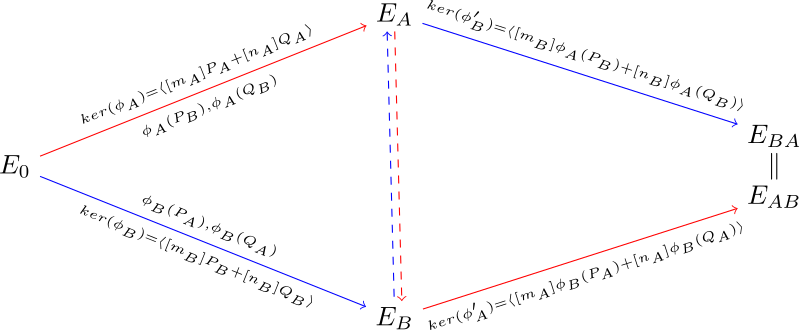
\includegraphics[scale=0.5]{keyexchange.png} % e.g. insert ./image for image.png in the working directory, adjust scale as necessary
\caption{SIDH key exchange between \alice \& \bob \cite{djp}}
\label{fig:kex} % insert suitable label, this is used to refer to a fig from within the text as shown above
\end{figure}

\subsection{Zero-Knowledge Proof of Identity}

Recall the earlier discussed notion of an identification scheme. A canonical identification scheme $\Pi_{\text{SID}} = (\textbf{KeyGen},\textbf{Prove},\textbf{Verify})$ can be derived somewhat analogously to the SIDH protocol, and is outlined in the original work of De Feo et al.

Say \bob has derived for himself the key pair $(\skb,\pkb)$ with $\skb = \{\mb,\nb\}$ and $\pkb = E_{\rb} = E_0/\langle [\mb]\genpb + [\nb]\genqb \rangle$ in relation to the public parameters $E_0$ and $\lbeb$. With $E_0$ and $E_{\rb}$ publicly known, $\Pi_{\text{ZKPoI}}$ revolves around \bob trying to prove to \alice that he knows the generator for $E_{\rb}$ without revealing it.

To achieve this, \bob internally mimicks an execution of the key exchange protocol $\Pi_{SIDH}$ with an arbitrary ``random" entity \randall.\\

\noindent
\textbf{KeyGen}: Key generation is performed exactly as in $\Pi_{\text{SIDH}}$, the only difference being that in $\Pi_{\text{ZKPoI}}$ only the prover (\bob, in our example,) needs to generate a keypair.\\

\noindent
\emph{Commitment}: \bob generates a random point $\cyr \in E_0[\laea]$ ($\cyr = [\mr]\genpa + [\nr]\genqa$) along with the corresponding isogenies necessary to compute the diagram below in full (if \alice were acting as the prover in $\Pi_{\text{ZKPoI}}$, then she would choose $\cyr \in E_0[\lbeb]$). \bob sends his commitment $com$ as $(com_1,com_2) = (E/\langle \cyr \rangle, E/\langle \rb, \cyr \rangle)$ to \alice.\\

\begin{center}
\begin{tikzpicture}
  \matrix (m) [matrix of math nodes,
               row sep=4em,
               column sep=4em,
               minimum width=2em] {
    E_0                     & E_0 / \langle \rb \rangle    \\
    E_0 / \langle \cyr \rangle & E_0 / \langle \rb, \cyr \rangle \\
  };
  \path[-stealth]
    (m-1-1) edge node [above] {$\pb$}  (m-1-2)
    (m-1-1) edge node [left]  {$\pr$}  (m-2-1)
    (m-2-1) edge node [below] {$\pbp$} (m-2-2)
    (m-1-2) edge node [right] {$\prp$} (m-2-2);
\end{tikzpicture}
\end{center}

\noindent
\emph{Response}: \alice chooses a bit $b$ at random and sends her challenge $ch = b$ to \bob.\\

\noindent
\textbf{Prove($sk$, $ch$)}: If \alice's challenge bit $ch = 0$ then \bob reveals the isogenies $\pr$ and $\prp$ (to do this, he can simply reveal the generators of the kernels of $\pr$ and $\prp$; $\cyr$ and $\pb(\cyr)$ respectively). This proves he knows the information necessary to form a shared secret with \randall \emph{if and only if} he happens to know the private key $\rb = \{[\mb]\genpb + [\nb]\genqb\}$. If $ch = 1$, \bob reveals the isogeny $\pbp$. This proves that \bob knows the information necessary to form a shared secret with \randall \emph{if and only if} he knows \randall's secret key $\cyr$.

In the following two graphs, bold arrows are used to indicate the information revealed by \bob. The graph on the left corresponds to \bob's actions when $ch = 0$, the graph on the right shows the information revealed when $ch = 1$.

\begin{center}
\begin{tikzpicture}[scale=.55]
	\begin{scope}[xshift=0cm]
		\matrix (m) [matrix of math nodes,
               row sep=4em,
               column sep=4em,
               minimum width=2em] {
    E_0                     & E_0 / \langle \rb \rangle    \\
    E_0 / \langle \cyr \rangle & E_0 / \langle \rb, \cyr \rangle \\
		};
		\draw[dashed] (m-1-1) edge node [above] {$\pb$}  (m-1-2);
		\draw[->, line width=2.0] (m-1-1) edge node [left]  {$\pr$}  (m-2-1);
		\draw[dashed] (m-2-1) edge node [below] {$\pbp$} (m-2-2);
		\draw[->, line width=2.0] (m-1-2) edge node [right] {$\prp$} (m-2-2);
	\end{scope}
	\begin{scope}[xshift=10cm]
		\matrix (m) [matrix of math nodes,
               row sep=4em,
               column sep=4em,
               minimum width=2em] {
    E_0                     & E_0 / \langle \rb \rangle    \\
    E_0 / \langle \cyr \rangle & E_0 / \langle \rb, \cyr \rangle \\
		};
		\draw[dashed] (m-1-1) edge node [above] {$\pb$}  (m-1-2);
		\draw[dashed] (m-1-1) edge node [left]  {$\pr$}  (m-2-1);
		\draw[->, line width=2.0] (m-2-1) edge node [below] {$\pbp$} (m-2-2);
		\draw[dashed] (m-1-2) edge node [right] {$\prp$} (m-2-2);
	\end{scope}
\end{tikzpicture}
\end{center}

Note that \bob cannot at once reveal all of the information necessary to convince \alice that he knows $\rb$. If he reveals $\cyr$, $\pb(\cyr)$, and $\pbp$ all in one go, he incidentally reveals his secret key $\rb = [\mb]\genpb + [\nb]\genqb$. This is because \bob reveals $\pbp$ by revealing the generator of $ker(\pbp)$, namely:
$$
(\rb, \cyr) = ([\mb]\genpb + [\nb]\genqb, [\mr]\genpa + [\nr]\genqa)
$$

How $\Pi_{\text{ZKPoK}}$ handles this is by having \bob and \alice run \textbf{Prove()} and \textbf{Verify()} for $\lambda$ iterations, with a different $(com, ch, resp)$ transcript generated for every instance. This way, if \bob is able to provide a $resp$ that satisfies \alice's $ch$ for every iteration, she can be sufficiently confident that \bob has knowledge of $\rb$. By taking this approach, \alice gains no knowledge of \bob's secret key (e.g. ``zero-knowledge").\footnote{This iterative approach to a zero-knowledge proof of knowledge is well illustrated by the "Ali Baba Cave" anecdote: \url{https://en.wikipedia.org/wiki/Zero-knowledge_proof\#Abstract_examples}.}\\

\noindent
\textbf{Verify($pk, com, ch$)}: Like the proving procedure, verification is a conditional function depending on the value of $b$:
\begin{itemize}
\item if $ch = 0$: return 1 \emph{if and only if} $\cyr$ and $\pb(\cyr)$ have order $\laea$ and generate the kernels of isogenies from $E_0 \rightarrow E_0/\langle \cyr \rangle$ and $E_0/\langle \rb \rangle \rightarrow E_0/\langle \rb, \cyr \rangle$ respectively.
\item if $ch = 1$: return 1 \emph{if and only if} $\pr(\rb)$ has order $\lbeb$ and generates the kernel of an isogeny over $E_0/\langle \cyr \rangle \rightarrow E_0/\langle \rb, \cyr \rangle$.
\end{itemize}

This scheme constitutes what is known in the literature as a \emph{zero knowledge} proof of identity. It is referred to as such because \alice, acting as the verifier, does not gain any information about \bob's secret key $sk$.

\section{Fiat-Shamir Construction}

The Fiat-Shamir construction (also frequently referred to as the Fiat-Shamir transform, or Fiat-Shamir hueristic,) is a high-level technique for transforming a canonical identification scheme into a secure  signature scheme.

The construction is rather simple. The idea is to first transform a given interactive identification protocol $\Pi_{\text{ID}}$ into a \emph{non-interactive} identification protocol. To achieve this, instead of allowing input from the verifier $\mathcal{V}$, we have our prover $\mathcal{P}$ generate the challenge $ch$ by itself. In order for the verifier to be able to check that $ch$ was generated honestly, we define $ch = H(com)$, where $H$ is some secure hash function. If we model $H$ as a random oracle, $H(com)$ is assumed truly random; from this it can be shown that it is just as difficult for an impersonator of $\mathcal{P}$ to find an accepting transcript $(com, H(com), resp)$ as it would be for them to successfully impersonate $\mathcal{P}$ in $\Pi_{\text{ID}}$.

Now that we've paired $\Pi_{\text{ID}}$ with $H$ to achieve a non-interactive identification scheme $\Pi_{\text{NID}}$, we need only to factor in some message $m$ from $\mathcal{P}$ to have constructed a signature scheme $\Pi_{\text{ID}}'$. This can be achieved by including $m$ in our calculation of the challenge: $ch = H(com, m)$. Therefore, given theorem \ref{thm:fiatshamir}, if $(com, H(com), resp)$ is an accepting transcript of $\Pi_{\text{NID}}$, then $(com, H(com, m), resp)$ is a secure signature for the message $m$. Of course, because $H(com, m)$ can be constructed by any passively observing party, it is redundant to include; and so $(com,resp)$ constitutes a valid signature for $m$. A proof of theorem \ref{thm:fiatshamir} can be found in \cite{sigs}. The security of the Fiat-Shamir construction was first proven by Pointcheval \& Stern in \cite{fsproof}.

\begin{tcolorbox}
\begin{theorem}[Fiat-Shamir Security]
\label{thm:fiatshamir}
Let $\Pi_{\text{ID}} = (\textbf{KeyGen}, \textbf{Commit}, \textbf{Prove}, \textbf{Verify})$ be a canonical identification scheme that is secure against a passive attack. Then, if $H$ is modeled as a random oracle, the signature scheme $\Pi_{\text{ID}}'$ that results from applying the Fiat-Shamir transform to $\Pi_{\text{ID}}$ is \emph{classically} existentially unforgeable under an adaptive chosen-message attack.
\end{theorem}
\end{tcolorbox}

We will write $\textbf{FS}(\Pi)$ to denote the result of applying the Fiat-Shamir transformation to some identification protocol $\Pi$.

\subsection{Unruh's Post-Quantum Adaptation}

In 2014, Ambainis et al. showed in \cite{rewinding} that classical security proofs for ``proof of knowledge" protocols are insecure in the quantum setting. This is due to a technique used in the proof of FST's security whereby the random oracle is subject to ``rewinding": the proof simulates multiple runs of FST with different responses from the random oracle \cite{rewinding}.

Following this insight, Unruh proposed in \cite{unruh} a construction based off that of Fiat \& Shamir which he proved to be secure in both the classical and quantum random oracle models.

Unruh's construction demands a small addition to the proof and verification procedures. In \textbf{Prove}, for every possible challenge value $ch_0, ch_1, ... , ch_n$, Unruh's construction demands that a hash of the corresponding responses $resp_0, resp_1, ... , resp_n$, along with the possible challenge values themselves, be included as input to the hash function $H$ computing the actual challenge. While Unruh originallly presented this technique in a generalized setting with $n$ possible challenge values, In figure \ref{unruhconst} we detail a version that assumes there are only two possible challenge values. This is done in an attempt to more closely reflect the zero-knowledge proof of identity scheme presented in \cite{djp}.

The construction is given in the form of two procedures: \textbf{Prove}$_{\textbf{Un}}$ and \textbf{Verify}$_{\textbf{Un}}$. Given the proving procedure \textbf{P}$_{\Pi}$ of some canonical identification scheme $\Pi$, \textbf{Prove}$_{\textbf{Un}}$ can be constructed and forms the basis for the \textbf{Sign} procedure of a quantum-safe signature scheme $\textbf{Un}(\Pi)$. Analagously, given the verification procedure \textbf{V}$_{\Pi}$ $\in \Pi$, \textbf{Verify}$_{\textbf{Un}}$ details the outline of signature verification in $\textbf{Un}(\Pi)$.

Similar to above, we will write $\textbf{Un}(\Pi)$ to denote the result of applying Unruh's construction to some identification protocol $\Pi$.

\begin{algorithm}
\caption{-- \textbf{Prove$_{\textbf{Un}}$(\textbf{P}$_{\Pi}$)}}\label{alg:unruhconst}
\begin{algorithmic}[1]
\If{$User$ = $\alice$}
	\State Pick a random point $S$ of order $\laea$
\EndIf
\If{$User$ = $\bob$}
	\State Pick a random point $S$ of order $\lbeb$
\EndIf
\State Compute the isogeny $\phi: E \rightarrow E/\langle S \rangle$
\State $pk \gets (E/\langle S \rangle, \phi(P_{User}), \phi(Q_{User}))$
\State $sk \gets S$
\State \Return ($sk$, $pk$)
\end{algorithmic}
\end{algorithm}

\begin{algorithm}
\caption{-- \textbf{Verify$_{\textbf{Un}}$(\textbf{V}$_{\Pi}$)}}\label{alg:unruhconst}
\begin{algorithmic}[1]
\If{$User$ = $\alice$}
	\State Pick a random point $S$ of order $\laea$
\EndIf
\If{$User$ = $\bob$}
	\State Pick a random point $S$ of order $\lbeb$
\EndIf
\State Compute the isogeny $\phi: E \rightarrow E/\langle S \rangle$
\State $pk \gets (E/\langle S \rangle, \phi(P_{User}), \phi(Q_{User}))$
\State $sk \gets S$
\State \Return ($sk$, $pk$)
\end{algorithmic}
\end{algorithm}

\section{Isogeny-based Signatures}
\label{sec:sigsbackground}

Since publication of the SIDH suite, there have been several attempts at providing authentication schemes using the same primitives. The post-quantum community had demonstrated undeniable signatures \cite{jvsig}, designated verifier signatures \cite{sunsig}, and undeniable blind signatures \cite{seshsig} all within the framework of isogeny-based systems. It was not until the work of Yoo et al. ((\cite{yoo})), however, that an isogeny-based protocol for general authentication was shown as demonstrably secure. This protocol, particularly its C implementation, is where we have decided to focus our efforts.

Now that we've seen the zero-knowledge proof of identity (ZKPoI) from \cite{djp} as well as Unruh's quantum-safe Fiat-Shamir adaption, we have presented all of the material necessary for an indepth analysis of the isogeny-based signature scheme presented by Yoo et al. The signature protocol, which we'll denote as $\Sigma'$, is an application of Unruh's construction to the SIDH ZKPoI. In this section we will refer to the SIDH ZKPoI as $\Sigma$.

$\Sigma'$ is defined in the traditional manner, by a tuple of algorithms for key generation, signing, and verifying: $\Sigma' = (\textbf{KeyGen()}, \textbf{Sign()}, \textbf{Verify()})$. \textbf{KeyGen()} in $\Sigma'$ is defined identically to the key generation found in SIDH key exchange. \textbf{Sign()} and \textbf{Verify()} are defined by applying Unruh's transformation to \textbf{Prove()} and \textbf{Verify()}.

For our discussion of the signature scheme, we will make use of the naming conventions used in Section 2.3. That is, we will discuss $\Sigma'$ as occuring between entities \bob and \alice, with \bob imitating the role of an arbitrary third party \randall during \textbf{Sign}.

The public parameters used in $\Sigma'$ are the same as outlined above for all of the protocols found in \cite{djp}. Namely, we have $p = \laea\lbeb \cdot f \pm 1$ where $\laea = 2$, $\lbeb = 3$, and $f$ is a cofacter such that $p$ is prime. We also set as parameter the curve $E$ such that $\#(E(F_{p^2})) = (\laea\lbeb)^2$. And again, we include the sets of points $\{\genpa, \genqa\}$ and $\{\genpb, \genqb\}$ generating $E[\laea]$ and $E[\lbeb]$ respectively. We have chosen $E$ over the previously used $E_0$ simply for ease of notation.

\subsection{Algorithmic Definitions}

It will be useful for us to outline in more detail the procedures of $\Sigma'$, at the very least to ease the transition into our discussion of the C implementation. In this subsection we will look at isogeny-level algorithmic definitions for \textbf{KeyGen()}, \textbf{Prove()}, and \textbf{Verify()}, and then look at how these procedures can be expressed in terms of the procedures of $\Pi_{\text{SIDH}}$.\\

\noindent
\textbf{KeyGen($\lambda$, $User$)}: As previously mentioned, key generation in $\Sigma'$ is identical to $\Sigma$:\textbf{KeyGen($\lambda$)}, which in turn is identical to $\Pi_{\text{SIDH}}$:\textbf{KeyGen($\lambda$)}. We've included a parameter $User$ equaling either $\alice$ or $\bob$ -- this denotes whether the user running the procedure uses \textcolor{blue}{blue} or \textcolor{red}{red} constants. We've also obfuscated the lower level details in regards to how points are generated and how isogenies can be constructed. We write $P_{User}$ and $Q_{User}$ for $\genpa$ \& $\genqa$ or $\genpb$ \& $\genqb$, depending on $User$.  The result is the following:

\begin{algorithm}
\caption{-- \textbf{KeyGen($\lambda$, $User$)}}\label{alg:keygensig}
\begin{algorithmic}[1]
\If{$User$ = $\alice$}
	\State Pick a random point $S$ of order $\laea$
\EndIf
\If{$User$ = $\bob$}
	\State Pick a random point $S$ of order $\lbeb$
\EndIf
\State Compute the isogeny $\phi: E \rightarrow E/\langle S \rangle$
\State $pk \gets (E/\langle S \rangle, \phi(P_{User}), \phi(Q_{User}))$
\State $sk \gets S$
\State \Return ($sk$, $pk$)
\end{algorithmic}
\end{algorithm}

\noindent
Transcribing this to the procedures of $\Pi_{\text{SIDH}}$ we arrive (quite trivially) at:\\

\begin{algorithm}
\caption{-- \textbf{KeyGen($\lambda$, $User$)} via $\Pi_{\text{SIDH}}$}\label{euclid}
\begin{algorithmic}[1]
\State ($sk$, $pk$) $\gets \Pi_{\text{SIDH}}$:\textbf{KeyGen($\lambda$, $User$)}
\State \Return ($sk$, $pk$)
\end{algorithmic}
\end{algorithm}

For \textbf{Sign($sk$, $m$)} and \textbf{Verify($pk$, $m$, $\sigma$)} we assume \bob to be the signer and \alice to be the verifier. Consequently, we will write the signer's key pair ($sk$, $pk$) as ($\rb$, $\pb$). Algorithms for which the roles are reversed can be constructed simply by replacing \textcolor{red}{red} constants with their \textcolor{blue}{blue} correspondants, and vice-versa.\\  

\noindent
\textbf{Sign($sk$, $m$)}: The sign procedure, as a consequence of the Unruh construction, makes use of two random oracle functions \textbf{H} and \textbf{G}. In the sign algorithm below, make note of how \bob computes both commitments and their corresponding responses for every iteration $i$ before he computes the challenge values (the bits of $J$). He then uses the $2\lambda$ bits of $J$ to decide which responses to include in $\sigma$.\\

\begin{algorithm}
\caption{-- \textbf{Sign($sk = \rb$, $m$)}}\label{euclid}
\begin{algorithmic}[1]
\For{\texttt{i = 1..2$\lambda$}}
	\State Pick a random point $\cyr$ of order $\laea$
	\State Compute the isogeny $\pr: E \rightarrow E/\langle \cyr \rangle$
	\State Compute the isogeny $\pbp : E/\langle \rb \rangle \rightarrow E/\langle \rb,\cyr \rangle$
	\State $(E_{1},E_{2}) \gets (E/\langle \cyr \rangle, E/\langle \cyr,\rb \rangle)$
	\State $com_{i} \gets (E_{1}, E_{2})$
	\State $ch_{i,0} \gets_{R} \{0,1\}$
	\State $ch_{i,1} \gets 1 - ch_{i,0}$
	\State $(resp_{i,0}, resp_{i,1}) \gets ((\cyr,\pb(\cyr)), \pr(\rb))$
	\If{$\texttt{ch}_{i,0} = 1$}
		\State \textbf{Swap($resp_{i,0}$,$resp_{i,1}$)}
	\EndIf
	\State $h_{i,j} \gets$ \textbf{G($resp_{i,j}$)}
\EndFor

\State $J_{1} \parallel ... \parallel J_{2\lambda} \gets$ \textbf{H($\pb$, $m$, $(com_{i})_{i}$,$(ch_{i,j})_{i,j}$,$(h_{i,j})_{i,j}$)}

\State \Return $\sigma \gets ((com_{i})_{i}, (ch_{i,j})_{i,j}, (h_{i,j})_{i,j}, (resp_{i,J_{i}})_{i})$
\end{algorithmic}
\end{algorithm}

\noindent
If we write out \textbf{Sign} using the $\Pi_{\text{SIDH}}$ API, we see that the only real computation is being performed by \textbf{KeyGen} and \textbf{SecAgr}, and our two random oracles \textbf{H} and \textbf{G}.  The rest of the algorithm is merely organizing the information we've generated into the transcript ($com$, $ch$, $resp$) and then finally into $\sigma$.

\begin{algorithm}
\label{alg:signvia}
\caption{-- \textbf{Sign($sk = \rb$, $m$)} via $\Pi_{\text{SIDH}}$}\label{euclid}
\begin{algorithmic}[1]
\For{\texttt{i = 1..2$\lambda$}}
	\State $(\cyr,\pr) \gets \Pi_{\text{SIDH}}$:\textbf{KeyGen($\lambda$, $\alice$)}
	\State $\pbp: E/\langle \rb \rangle \rightarrow E/\langle \rb,\cyr \rangle \gets \Pi_{\text{SIDH}}$:\textbf{SecAgr($\rb$, $\pr$)}
	\State $(E_{1},E_{2}) \gets (E/\langle \cyr \rangle, E/\langle \rb,\cyr \rangle)$
	\State $com_{i} \gets (E_{1}, E_{2})$
	\State $ch_{i,0} \gets_{R} \{0,1\}$
	\State $ch_{i,1} \gets 1 - ch_{i,0}$
	\State $(resp_{i,0}, resp_{i,1}) \gets ((\cyr,\pb(\cyr)), \pr(\rb))$
	\If{$\texttt{ch}_{i,0} = 1$}
		\State \textbf{Swap($resp_{i,0}$,$resp_{i,1}$)}
	\EndIf
	\State $h_{i,j} \gets$ \textbf{G($resp_{i,j}$)}
\EndFor

\State $J_{1} \parallel ... \parallel J_{2\lambda} \gets$ \textbf{H($\pb$, $m$, $(com_{i})_{i}$,$(ch_{i,j})_{i,j}$,$(h_{i,j})_{i,j}$)}

\State \Return $\sigma \gets ((com_{i})_{i}, (ch_{i,j})_{i,j}, (h_{i,j})_{i,j}, (resp_{i,J_{i}})_{i})$
\end{algorithmic}
\end{algorithm}


\noindent
\textbf{Verify($pk$, $m$, $\sigma$)}: \alice begins her execution of \textbf{Verify()} where \bob ended his execution of \textbf{Sign()}, with the computation of $J$. \alice then knows at each iteration what check to perform on \bob's response, based on a conditional branch. You will notice that \bob's secret key $\rb$ occurs in the negative path of this branch; this is not a security concern because it is actually the point $\pr(\rb)$ that is communicated in $\sigma$, from which $\rb$ cannot be recovered.\\

\begin{algorithm}[H]
\caption{-- \textbf{Verify($pk = \pb$, $m$, $\sigma$)}}\label{euclid}
\begin{algorithmic}[1]
\State Parse $((com_i)_i, (ch_{i,j})_{i,j}, (h_{i,j})_{i,j}, (resp_{i})_{i}) \gets \sigma$
\State $J_{1} \parallel ... \parallel J_{2\lambda} \gets$ \textbf{H($\pb$, $m$, $(com_{i})_{i}$,$(ch_{i,j})_{i,j}$,$(h_{i,j})_{i,j}$)}
\For{\texttt{i = 0..2$\lambda$}}
	\State \textbf{check} $h_{i,J_{i}} = G(resp_{i})$
	\If{$ch_{i,J_{i}} = 0$}
		\State Parse $(\cyr,\pb(\cyr)) \gets resp_{i}$
		\State \textbf{check} $(\cyr, \pb(\cyr))$ have order $\laea$
		\State \textbf{check} $\cyr$ generates the kernel of the isogeny $E \rightarrow E_{1}$
		\State \textbf{check} $\pb(\cyr)$ generates the kernel of the isogeny $E/\langle \rb \rangle \rightarrow E_{2}$
	\Else
		\State Parse $\pr(\rb) \gets resp_{i}$
		\State \textbf{check} $\pr(\rb)$ has order $\lbeb$
		\State \textbf{check} $\pr(\rb)$ generates the kernel of the isogeny $E_{1} \rightarrow E_{2}$
	\EndIf
\EndFor

\If{all checks succeed}
	\State \Return 1
\Else
	\State \Return 0
\EndIf
\end{algorithmic}
\end{algorithm}

\noindent
What we are checking for in the verification process is whether or not \bob and \randall performed an honest and valid key exchange. And so, if the challenge bit is 0, we can use SIDH key generation to determine that $\cyr$ and $\pr$ are a valid key pair and then run SIDH secret agreement with $\cyr$ and \bob's public key $\pb$ to confirm that it properly executes outputting an isogeny with kernel generated by $\pb(\cyr)$. If the challenge bit is 1, we can run an instance of SIDH secret agreement to verify that $\pr(\rb)$ generates the kernel of an isogeny with domain $E_{1}$ and co-domain $E_{2}$ (refer again to the diagrams outlining \textbf{Prove} of section 2.3.2).

These observations are formalized in Algorithm 6, where we rewrite $\Sigma'$:\textbf{Verify()} in terms of $\Pi_{\text{SIDH}}$ procedure calls. Note, in line 10 of Algorithm 6, the call $\Pi_{\text{SIDH}}$:\textbf{SecAgr($\pr(\rb)$, $\pr$)}. It should be noted that $\pr(\rb)$ is not the proper secret key input used by \bob in \textbf{Sign()}, but we will see in the section to follow how we can use $\pr(\rb)$ in the C implementation of \textbf{SecAgr} to perform our verification (without compromising \bob's secret key $\rb$).

\begin{algorithm}[H]
\caption{-- \textbf{Verify($pk = \pb$, $m$, $\sigma$)} via $\Pi_{\text{SIDH}}$}\label{euclid}
\begin{algorithmic}[1]
\State Parse $((com_i)_i, (ch_{i,j})_{i,j}, (h_{i,j})_{i,j}, (resp_{i})_{i}) \gets \sigma$
\State $J_{1} \parallel ... \parallel J_{2\lambda} \gets$ \textbf{H($\pb$, $m$, $(com_{i})_{i}$,$(ch_{i,j})_{i,j}$,$(h_{i,j})_{i,j}$)}
\For{\texttt{i = 0..2$\lambda$}}
	\State \textbf{check} $h_{i,J_{i}} = G(resp_{i,J_{i}})$
	\If{$ch_{i,J_{i}} = 0$}
		\State Parse $(\cyr,\pb(\cyr)) \gets resp_{i,J_{i}}$
		\State \textbf{check} $(\cyr, \pr)$ is a valid output of $\Pi_{\text{SIDH}}$:\textbf{KeyGen($\lambda$, $\alice$)}
		\State \textbf{check} that $\Pi_{\text{SIDH}}$:\textbf{SecAgr($\cyr$, $\pb$)} successfully outputs an isogeny with co-domain $E_{2}$
	\Else
		\State Parse $\pr(\rb) \gets resp_{i,J_{i}}$
		\State \textbf{check} that $\Pi_{\text{SIDH}}$:\textbf{SecAgr($\pr(\rb)$, $\pr$)} successfully outputs an isogeny with co-domain $E_{2}$
	\EndIf
\EndFor

\If{all checks succeed}
	\State \Return 1
\Else
	\State \Return 0
\EndIf
\end{algorithmic}
\end{algorithm}

\section{Implementations of Isogeny-based Cryptographic Protocols}
\label{sec:implementations}

Having now introduced all of the background material necessary for understanding SIDH and the isogeny-based signature scheme in detail, we will investigate the portions of the SIDH C library which are relevent to our contributions.

The SIDH C library, written by a research team at Microsoft Research, was released in 2016 alongside an article titled \emph{Efficient Algorithms for Supersingular Isogeny Diffie-Hellman} (see \cite{effalg}). The article in question details several adjustments to the algorithms and data-representations outlined in \cite{djp}, leading to improved performance and key-sizes. Their library (which we will henceforth refer to as \sidh) consists of C and assembly implementations of the algorithms outlined in \cite{effalg}. Much of these functions are tailored to a specific set of parameters allowing for increased performance. The library presents 128-bit quantum security and 192-bit classical security key exchange up to 2.9 times faster than any previous isogeny-based key-exchange system. We will look at some of the details of \sidh below. 

Before proceeding, it may be advisable to briefly review the section on notation (\ref{sub:notation}) if one has not already.

\subsection{Parameters \& Data Representation}
\label{subsec:datarep}

\noindent
\emph{Parameters}. \sidh operates over the underlying basefield $\mathbb{F}_{p}$ where $p = \laea\cdot\lbeb - 1$, with $\la = 2$, $\lb = 3$, $\ea = 372$, and $\eb = 239$, giving $p$ a bitlength of 751. Now, recall the Montgomery representation of a curve:
$$
By^2 = Cx^3 + Ax^2 + Cx
$$

\sidh uses the public parameter curve $E$ defined in Montgomery form with $A = 0$, $B = 1$, and $C = 1$. The point pairs ($\genpa,\genqa$) and ($\genpb, \genqb$), generating $E[\laea]$ and $E[\lbeb]$ respectively, are hard-coded as an array of bytes. These parameters (including related data such as the bitlength of certain constants) are stored in the struct type \code{CurveIsogenyStaticData} under the variable name \code{SIDHp751}. This struct, along with many other \sidh data types and representations, will be outlined in the coming subsection.

One priority of the parameter choices found in \code{SIDHp751} was to approach $\laea \approx \lbeb$. This attempted at balancing $\laea$ and $\lbeb$ helps to ensure two things: first, that no side of the key exchange is any easier to attack than the other, and second, that the cost of computation is split evenly between parties. This constraint had to be compromise with the primary security concern: that $p$ must have a bit-length providing sufficient classical and quantum security.\\

\noindent
\emph{Data Structures}. There are several custom-defined data structures that are integral to \sidh. Below, we will briefly cover the ones which are likely to arise in our discussion:\\

\emph{Field elements}
\begin{itemize}
	\item \code{felm\_t} -- buffer of bytes representing elements of $\mathbb{F}_{p}$.
	\item \code{f2elm\_t} -- pair of \code{felm\_t} representing elements of $\mathbb{F}_{p^2}$.
\end{itemize}

\emph{Elliptic curve points}
\begin{itemize}
	\item \code{point\_affine} -- an \code{f2elm\_t} \code{x} and an \code{f2elm\_t} \code{y} representing a point in affine space.
	\item \code{point\_proj} -- an \code{f2elm\_t} \code{X} and an \code{f2elm\_t} \code{Z} representing a point as projective XZ Montgomery coordinates.
	\item \code{point\_full\_proj} -- \code{f2elm\_t} elements \code{X}, \code{Y}, and \code{Z} representing a point in projective space.
	\item \code{point\_basefield\_affine} -- an \code{felm\_t} \code{x} and an \code{felm\_t} \code{y} representing a point in affine space over the base field.
	\item \code{point\_basefield\_proj} -- an \code{felm\_t} \code{X} and an \code{felm\_t} \code{Z} representing a point as projective XZ Montgomery coordinates over the base field.
\end{itemize}

\emph{Cryptographic structures}
\begin{itemize}
	\item \code{publickey\_t} -- three \code{f2elm\_t}s representing a public key.\\
	\code{publickey\_t[0]} = user's private isogeny applied to the other party's generator $P_x$\\
	\code{publickey\_t[1]} = user's private isogeny applied to the other party's generator $Q_x$\\
	\code{publickey\_t[2]} = user's private isogeny applied to $P_x - Q_x$
\end{itemize}

\emph{Curve structures}
\begin{itemize}
	\item \code{CurveIsogenyStruct} -- Structure containing all necessary public parameter data.
	\item \code{CurveIsogenyStaticData} -- The same as \code{CurveIsogenyStruct}, but with buffer sizes fixed for \code{SIDHp751}.
\end{itemize}

The reader may note that \code{publickey\_t} does not contain any information defining the user's co-domain curve $E/\langle S \rangle$ (with $S$ as the users secret key). It just so happens that in $\Pi_{\text{SIDH}}$ key exchange, the curves $E/\langle \ba \rangle$ and $E/\langle \rb \rangle$ are simply intermediary steps (useful for conceptualizing the protocol) and not necessary for computing the shared secret $j(E_{\ba\rb})$. 

Also worth noting is the lack of a specific data structure for representing curves. As it turns out, curves within $\Pi_{\text{SIDH}}$ can be distinctly represented by their $A$ value alone. As we are working with curves defined over $\mathbb{F}_{p^2}$, we have $A \in \mathbb{F}_{p^2}$ and thus we can succinctly represent any curve with a single \code{f2elm\_t}. 

\subsection{\sidh Design Decisions}
\label{subsec:design}

The following are, at a high-level, the algorithmic improvements upon $\Pi_{\text{SIDH}}$ as outlined in \cite{effalg}. Costella et al. do make additional contributions in their paper, however we will discuss only those contributions which pertain to the performance of SIDH.\\

\noindent
\emph{Projective Space Arithmetic}. As is common in ECC, a vast majority of the procedures of \sidh operate over elliptic curve points which are defined over \emph{projective space} (recall Section \ref{snip:projspace}). This widely-deployed technique is used to avoid the substantial cost of field element inversions (computing $x^{-1}$ for some element $x \in \mathbb{F}_{p^2}$). This means the majority of our calculations are performed over \code{point\_proj} structures using \emph{Montgomery arithmetic} (Section \ref{snip:montgomery}) and converted to \code{point\_affine} when necessary. This general design strategy is highly related to our first contribution, which will be elaborated upon in Section \ref{sec:batching}.

In addition to traditional point-wise projective arithmetic, Costella et al. showed that isogeny arithmetic can also be carried out in this space. By performing isogeny arithmetic in the projective space, the number of $\mathbb{F}_{p^2}$ inversions in $\Pi_{\text{SIDH}}$:\textbf{KeyGen} and $\Pi_{\text{SIDH}}$:\textbf{SecAgr} can be reduced to 1 and 2, respectively.\\

\noindent
\emph{Key Representation}. Recall the origin of an $\Pi_{\text{SIDH}}$ private key $(m, n)$: the goal is to randomly select a generator of the torsion group $E[\laea]$ (or $E[\lbeb]$ for \bob). It is noted in \cite{djp} that any generator of the required torsion group is sufficient. It is also noted that $m$, unless equal to the order of the torsion group, is invertible. Because of this, \alice, for example, can simple compute $R = \genpa + [m^{-1}n]\genqa$, thus enabling secret keys to be stored as a single $\mathbb{F}_{p^2}$ element (which is referred to as $m$). This technicality has been implemented in \sidh, which both saves on storage as well as offers a means for generating secret keys that is more efficient than the trivial scalar multiplication and point-wise addition approach to computing $[m]P + [n]Q$.\\

\noindent
\emph{Tailor-made Montgomery Multiplication}. The parameters of a default \sidh execution, stored in \code{SIDHp752}, support efficient arithmetic and grant access to a variety of modular arithmetic optimizations. These optimizations inlude esfs,esdfsef,sefsef.. Moreover, Costella et al. supply a modified version of the Montgomery multiplication algorithm which, when performing over the class of curves outlined by their set of parameters, yields faster modular arithmetic.  

\subsection{Key Exchange \& Critical Functions}
\label{subsec:functions}

There are 3 central modules (C files) in \sidh, all dealing with different levels of abstraction in the $\Pi_{\text{SIDH}}$ protocol.  Figure \ref{fig:halfmap} illustrates the relationship between these modules and the abstraction levels of isogeny-based key exchange. 

Operating at the lowest abstraction level is the module \code{fpx.c}, wherein functions for manipulating $\mathbb{F}_{p}$ and $\mathbb{F}_{p^2}$ elements are defined. One level up from \code{fpx.c} we have \code{ec\_isogeny.c}, containing functions pertaining to elliptic curves and point arithmetic (such as \code{j\_inv(...)} for computing the j-invariant of a curve and \code{secret\_pt(...)} for computing a users secret point $S$ given their private key $m$). The final, highest abstraction-level module we will discuss is \code{kex.c}. \code{kex.c} contains the protocol-level functions for performing $\Pi_{\text{SIDH}}$, namely \code{KeyGeneration\_A(...)} and \code{KeyGeneration\_B(...)} for generating \alice and \bob's private and public keys, as well as \code{SecretAgreement\_A(...)} and \code{SecretAgreement\_B(...)} for completing the secret agreement from both sides of the key exchange.

\begin{figure}[!htb]
\centering
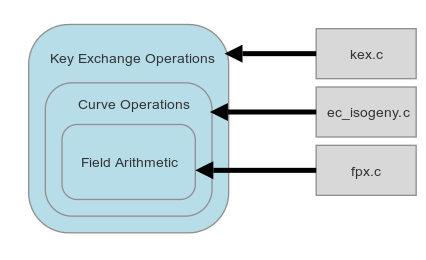
\includegraphics[scale=0.7]{halfmapwcurve.png} % e.g. insert ./image for image.png in the working directory, adjust scale as necessary
\caption{Relationship between $\Pi_{\text{SIDH}}$ \& \sidh modules}
\label{fig:halfmap} % insert suitable label, this is used to refer to a fig from within the text as shown above
\end{figure}

For functions defined in \code{fpx.c} the notational practice is to prepend function names with either \code{fp} or \code{fp2}, signifying whether the function is defined for elements of $\mathbb{F}_{p}$ or $\mathbb{F}_{p^2}$. Additionally, it is common to append \code{\_mont} to the name of functions which utilize Montgomery arithmetic, and thus expect elements in Montgomery representation. Functions in \code{fpx.c} are largely defined by byte and memory arithmetic, with the exception of slightly higher-level functions (such as field element inversion, \code{fpinv751\_mont(...)}) which are defined in terms of other \code{fpx.c} functions. Furthermore, for efficiency, functions of \code{fpx.c} are defined as \code{\_\_inline} when applicable.

In addition to the \code{fpx.c} functions we've outlined in Figure \ref{fig:fpfuncs} there are of course definitions for addition, copying elements, retrieving the zero element, Montgomery multiplication, squaring, and so on and so forth. 

\begin{figure}
\begin{center}
\code{fpx.c} functions\\
\begin{tabular}{|c|c|c|}
	\toprule
	Function & Input & Output\\
	\hline
	\code{to\_fp2mont} & \code{f2elm\_t a} & \code{f2elm\_t ma}\\
	Converts an $\mathbb{F}_{p^2}$  element & &\\
	to Montgomery representation & &\\
	\hline
	\code{from\_fp2mont} & \code{f2elm\_t ma} & \code{f2elm\_t a}\\
	Converts an $\mathbb{F}_{p^2}$ element & &\\
	from Montgomery representation  & &\\
	to regular form & &\\
	\hline
	\code{fp2inv751\_mont\_bingcd} & \code{f2elm\_t a} & \code{f2elm\_t a}$^{-1}$\\
	performs \emph{non-constant} & &\\
	time inversion of & &\\
	a $\mathbb{F}_{p^2}$ element & &\\
	\hline
	\code{fp2inv751\_mont} & \code{f2elm\_t a} & \code{f2elm\_t a}$^{-1}$\\
	performs \emph{constant} & &\\
	time inversion of & &\\
	a $\mathbb{F}_{p^2}$ element & &\\
	\bottomrule
\end{tabular}
\end{center}
\label{fig:fpfuncs}
\end{figure}

\code{ec\_isogeny.c} functions are defined almost exclusively in terms of \code{fpx.c} functions, with a few occurances of internal function calling. Functions in this module that are significant to our our work are briefly summerized in Figure \ref{fig:ecfuncs}. The implementation specifics of most other \code{ec\_isogeny.c} functions are not critical to our work, and so have been excluded. The design and efficiency of these algorithms do, however, have a rich background and can be further read about in \cite{djp} and \cite{effalg}.

\begin{figure}
\begin{center}
\code{ec\_isogeny.c} functions\\
\begin{tabular}{|c|c|c|}
	\toprule
	Function & Input & Output\\
	\hline
	\code{j\_inv} & \code{f2elm\_t A} & \code{f2elm\_t jinv}\\
	computes the j-invariant & \code{f2elm\_t C} &\\
	of a curve with represented & &\\
	in Montgomery form with \code{A} and \code{C} & &\\
	\hline
	\code{secret\_pt} & \code{point\_basefield P} & \code{point\_proj R}\\
	generates the secret & \code{digit\_t m} &\\
	point \code{R} from & \code{SIDHp751} &\\
	secret key \code{m} & \code{int AliceOrBob} &\\
	\hline
	\code{inv\_3\_way} & \code{f2elm\_t z1} & \code{f2elm\_t z1}$^{-1}$\\
	performs simultaneous inversion & \code{f2elm\_t z2} & \code{f2elm\_t z2}$^{-1}$\\
	of three elements & \code{f2elm\_t z3} & \code{f2elm\_t z3}$^{-1}$\\
	\hline
	\code{inv\_4\_way} & \code{f2elm\_t z1} & \code{f2elm\_t z1}$^{-1}$\\
	performs simultaneous inversion & \code{f2elm\_t z2} & \code{f2elm\_t z2}$^{-1}$\\
	of 4 elements & \code{f2elm\_t z3} & \code{f2elm\_t z3}$^{-1}$\\
	& \code{f2elm\_t z4} & \code{f2elm\_t z4}$^{-1}$\\
	\hline
	\code{generate\_2\_torsion\_basis} & \code{f2elm\_t A} & \code{point\_full\_proj R1}\\
	constructs a basis ($\{R1, R2\}$) & \code{SIDHp751} & \code{point\_full\_proj R2}\\
	generating $E[\laea]$ &  &\\
	\hline
	\code{generate\_3\_torsion\_basis} & \code{f2elm\_t A} & \code{point\_full\_proj R1}\\
	constructs a basis ($\{R1, R2\}$) & \code{SIDHp751} & \code{point\_full\_proj R2}\\
	generating $E[\lbeb]$ & &\\
	\bottomrule
\end{tabular}
\end{center}
\label{fig:ecfuncs}
\end{figure}

The key exchange procedures found in \code{kex.c} are composed entirely of calls to \code{fpx.c} and \code{ec\_isogeny.c} functions, modulo some basic branching logic. All of the functions from this module are relevant to our work - we provide quick debriefings of these functions in Figure \ref{fig:kexfuncs}.

\begin{figure}
\begin{center}
\code{kex.c} functions\\
\begin{tabular}{|c|c|c|}
	\toprule
	Function & Input & Output\\
	\hline
	\code{KeyGeneration\_A} & \code{unsigned char* privateKeyA} & \code{unsigned char* privateKeyA} \\
	performs key generation & \code{bool generateRandom} & \code{unsigned char* publicKeyA} \\
	for \alice & &\\
	\hline
	\code{KeyGeneration\_B} & & \code{unsigned char* privateKeyB}\\
	performs key generation & & \code{unsigned char* publicKeyB}\\
	for \bob & &\\
	\hline
	\code{SecretAgreement\_A} & \code{unsigned char* privateKeyA} & \code{unsigned char* sharedSecretA}\\
	computes the shared secret & \code{unsigned char* publicKeyB} & \code{point\_proj kerngen}\\
	from \alice's perspective & \code{point\_proj kerngen} &\\
	\hline
	\code{SecretAgreement\_B} & \code{unsigned char* privateKeyB} & \code{unsigned char* sharedSecretB}\\
	computes the shared secret & \code{unsigned char* publicKeyA} & \code{point\_proj kerngen}\\
	from \bob's perspective & \code{point\_proj kerngen} &\\
	\bottomrule
\end{tabular}
\end{center}
\label{fig:kexfuncs}
\end{figure}

The reader may note that, in Figure \ref{fig:kexfuncs}, \code{privateKeyA} (in \code{KeyGeneration\_A}) and \code{kerngen} (in both secret agreements) appear as both inputs and outputs. This is not a mistake. In \code{KeyGeneration\_A}, if \code{generateRandom = false} is passed as an input, then \code{privateKeyA} is expected to be set, and the corresponding public key is computed. In secret agreement, if \code{kerngen} is set to null then the algorithm proceeds normally. If it is set to a valid point, however, it can be used in place of a secret key input (which in such a case is expected to be null). Both of these details are critical to the design of signature functions as they are described below.

\subsection{Signature Layer}
\label{subsec:sigcode}

Yoo et al. provided, along with their publication of \cite{yoo}, an implementation of their signature scheme as a fork to \sidh. All of their functions are written specifically for an instance of $\Sigma'$ where the signer is assuming the \rb role (meaning that \randall assumes the \ba role), but their algorithms could be trivially modified to provide versions supporting a signer in the \ba role. Their contributions to the \sidh codebase come in the form of the functions listed below.

\begin{figure}
\begin{center}
\begin{tabular}{|c|c|c|c|}
	\toprule
	Function & Input & Output\\
	\midrule
	\code{isogeny\_keygen} & & \code{unsigned char* privateKeyB}\\
	generates the signers & & \code{unsigned char* publicKeyB}\\
	key pair & &\\
	\hline
	\code{isogeny\_sign} & \code{privateKey} & \code{Signature sig}\\
	produces a signature & \code{publicKey} &\\
	for a message & message $m$ &\\
	\hline
	\code{sign\_thread} & & \\
	performs a single iteration & &\\
	of the for-loop in \textbf{Sign} & &\\
	\hline
	\code{isogeny\_verify} & \code{Signature sig} & \code{true} or \code{false}\\
	checks the validity & &\\
	of a signature & &\\
	\hline
	\code{verify\_thread} & &\\
	performs a single iteration & &\\
	of the for-loop in \textbf{Verify} & &\\
	\bottomrule
\end{tabular}
\end{center}
\label{fig:sigfuncs}
\end{figure}

To begin, \code{isogeny\_keygen} has a trivial definition; \code{KeyGeneration\_B} is called and populates the signer's public and private keys. \code{isogeny\_keygen} returns the success status of the call to \code{KeyGeneration\_B}.

In their original fork of \sidh, Yoo et al. included these functions in the file \code{kex\_tests.c}. This file was originally intended for testing the functions of \code{kex.c}, and so our fork of the library has placed the signature functions in a new file \code{SIDH\_signature.c}. We have also included a file \code{sig\_tests.c} for testing the contents and performance of \code{SIDH\_signature.c} functions. 

If we transcribe the procedures $\Sigma'$:\textbf{Sign} and $\Sigma'$:\textbf{Verify} (as described in Section \ref{subsec:sigsbackground}) to the language of the \sidh API, we have in essence the procedures \code{Sign} and \code{Verify} given by Algorithms \ref{alg:signcode} and \ref{alg:verifcode} respectively.\\

\begin{algorithm}
\caption{-- \code{Sign($sk_{\rb}$, $m$)}}\label{alg:signcode}
\begin{algorithmic}[1]
\For{\texttt{i = 1..2$\lambda$}}
	\State $(sk_{\cyr} = \cyr, pk_{\cyr}) \gets \code{KeyGeneration\_A(\code{NULL}, \code{true})}$
	\State $(E/\langle \rb,\cyr \rangle, \pr(\rb)) \gets \code{SecretAgreement\_B(}sk_{\rb}, pk_{\cyr}, \code{NULL})$
	\State $(E_{1},E_{2}) \gets (E/\langle \cyr \rangle, E/\langle \rb,\cyr \rangle)$
	\State $(\texttt{com}[i]_{0}, \texttt{com}[i]_{1}) \gets (E_{1}, E_{2})$
	\State $(\texttt{resp}[i]_{0}, \texttt{resp}[i]_{1}) \gets (\cyr, \pr(\rb))$
	\State $h[i] \gets$ \code{keccak(resp$[i]_0$)|keccak(resp$[i]_1$)}
\EndFor

\State $J_{1} \parallel ... \parallel J_{2\lambda} \gets$ \code{keccak(com, $m$, $h$)}

\State \Return $\sigma \gets ((\texttt{com}_{i})_{i}, (\texttt{ch}_{i,j})_{i,j}, (h_{i})_{i}, ((\texttt{resp})[J_{i}])$
\end{algorithmic}
\end{algorithm}

\begin{algorithm}[H]
\caption{-- \code{Verify($pk = \pb$, $m$, $\sigma$)}}\label{alg:verifcode}
\begin{algorithmic}[1]
\State $J_{1} \parallel ... \parallel J_{2\lambda} \gets$ \code{keccak(com, $m$, $h$)}
\For{\texttt{i = 0..2$\lambda$}}
	\State \textbf{check} $h[i] =$ \code{keccak(resp$[i]_0$)|keccak(resp$[i]_1$)}
	\If{$J_{i} = 0$}
		\State $\cyr \gets \code{resp}[i]_{0}$
		\State $pk_{\cyr} \gets$ \code{KeyGeneration\_A(\cyr, \code{false})}
		\State \textbf{check} $pk_{\cyr}$ = \code{com$[i]_{0}$}
		\State $E_{\cyr\rb} \gets$ \code{SecretAgreement\_A($\cyr$, $\pb$, NULL)}
		\State \textbf{check} $E_{\cyr\rb}$ = \code{com$[i]_{1}$}
	\Else
		\State $\pr(\rb) \gets \code{resp}[i]_{1}$
		\State $pk_{\cyr} \gets \code{com}[i]_{0}$
		\State $E_{\rb\cyr} \gets$ \code{SecretAgreement\_B(NULL, $pk_{\cyr}$, $\pr(\rb)$)}
		\State \textbf{check} $E_{\rb\cyr}$ = \code{com$[i]_{1}$}
	\EndIf
\EndFor

\If{all checks succeed}
	\State \Return 1
\Else
	\State \Return 0
\EndIf
\end{algorithmic}
\end{algorithm}

Outside of simply replacing $\Pi_{\text{SIDH}}'$ procedure calls with \sidh functions, the reader may notice additional differences between \code{Sign} and \code{Verify} and their $\Sigma'$ counterparts. Namely, Yoo et al. have chosen to exclude the challenge bit $ch$ in the \sidh implementations of these functions, consequently excluding the conditional and \textbf{Swap} statement of lines 8 and 9 in Algorithm 4. 


